\documentclass{article}
\usepackage{fullpage}
\usepackage{indentfirst}
\usepackage{amsmath}
\usepackage{amsfonts}
\usepackage{array}
\usepackage{tipa}
\usepackage{tikz}
\usepackage{tikz-qtree}
\usetikzlibrary{matrix, arrows, automata}
\usepackage{gb4e}
\noautomath
\newcommand{\Y}{$\checkmark$}
\newcommand{\N}{\ding{55}}
\newcommand{\R}{$\Rightarrow$}
\newcommand\myeq{\mathrel{\stackrel{\makebox[0pt]{\mbox{\normalfont\tiny def}}}{=}}}
\title{Contour Shift in Zhenhai}
\author{Chris Oakden}
\begin{document}
\maketitle
Chen (2000), citing Rose (1990), presents data from Zhenhai, an Wu dialect spoken in Zhejiang. He argues that Zhenhai sandhi provides evidence for contour shift/spreading independent of register, and therefore motivates separate register and contour nodes in representation. Chen's assessment is that this pattern is predicted by Bao's tonal geometry but not Yip's. \par
Abstracting away from certain details, the contour shifting pattern /LM.HL/ $\mapsto$ [L.MH] can be represented as in the figure below:
\begin{center}
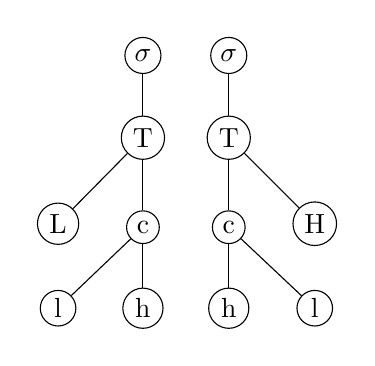
\begin{tikzpicture} [baseline = (y1.base)]
\matrix (m) [matrix of nodes, column sep = 1.5em, row sep = 1.5em]{
& \node[draw,circle, inner sep =2pt](x1){$\sigma$};  &  \node[draw,circle, inner sep =2pt](x2){$\sigma$};  \\
& \node[draw,circle, inner sep =2pt](y1){T}; &   \node[draw,circle, inner sep =2pt](y2){T}; \\
\node[draw,circle, inner sep =2pt](z1){L}; & \node[draw,circle, inner sep =2pt](z2){c}; &   \node[draw,circle, inner sep =2pt](z3){c}; & \node[draw,circle, inner sep =2pt](z4){H}; \\
\node[draw,circle, inner sep =2pt](t1){l}; & \node[draw,circle, inner sep =2pt](t2){h}; &  \node[draw,circle, inner sep =2pt](t3){h}; & \node[draw,circle, inner sep =2pt](t4){l}; \\
};
\draw (x1) -- (y1);
\draw (x2) -- (y2);
\draw (z1) -- (y1);
\draw (z2) -- (y1);
\draw (z2) -- (t1);
\draw (z2) -- (t2);
\draw (y2) -- (z3);
\draw (y2) -- (z4);
\draw (z3) -- (t3);
\draw (z3) -- (t4);
\end{tikzpicture}
\hspace{.3cm}
$\rightarrow$
\hspace{.3cm}
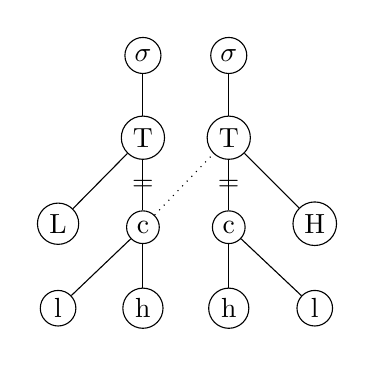
\begin{tikzpicture} [baseline = (y1.base)]
\matrix (m) [matrix of nodes, column sep = 1.5em, row sep = 1.5em]{
& \node[draw,circle, inner sep =2pt](x1){$\sigma$};  &  \node[draw,circle, inner sep =2pt](x2){$\sigma$};  \\
& \node[draw,circle, inner sep =2pt](y1){T}; &   \node[draw,circle, inner sep =2pt](y2){T}; \\
\node[draw,circle, inner sep =2pt](z1){L}; & \node[draw,circle, inner sep =2pt](z2){c}; &   \node[draw,circle, inner sep =2pt](z3){c}; & \node[draw,circle, inner sep =2pt](z4){H}; \\
\node[draw,circle, inner sep =2pt](t1){l}; & \node[draw,circle, inner sep =2pt](t2){h}; &  \node[draw,circle, inner sep =2pt](t3){h}; & \node[draw,circle, inner sep =2pt](t4){l}; \\
};
\draw (x1) -- (y1);
\draw (x2) -- (y2);
\draw (z1) -- (y1);
\path (z2) edge node{=} (y1);
\draw (z2) -- (t1);
\draw (z2) -- (t2);
\path (z3) edge node{=} (y2);
\draw (y2) -- (z4);
\draw (z3) -- (t3);
\draw (z3) -- (t4);
\draw [dotted] (z2) -- (y2);
\end{tikzpicture}
\hspace{.3cm}
$\rightarrow$
\hspace{.3cm}
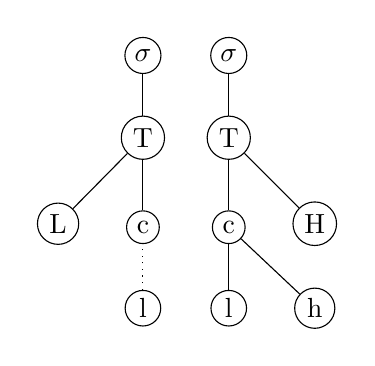
\begin{tikzpicture} [baseline = (y1.base)]
\matrix (m) [matrix of nodes, column sep = 1.5em, row sep = 1.5em]{
& \node[draw,circle, inner sep =2pt](x1){$\sigma$};  &  \node[draw,circle, inner sep =2pt](x2){$\sigma$};  \\
& \node[draw,circle, inner sep =2pt](y1){T}; &   \node[draw,circle, inner sep =2pt](y2){T}; \\
\node[draw,circle, inner sep =2pt](z1){L}; & \node[draw,circle, inner sep =2pt](z2){c}; &   \node[draw,circle, inner sep =2pt](z3){c}; & \node[draw,circle, inner sep =2pt](z4){H}; \\
& \node[draw,circle, inner sep =2pt](t1){l}; &  \node[draw,circle, inner sep =2pt](t3){l}; & \node[draw,circle, inner sep =2pt](t4){h}; \\
};
\draw (x1) -- (y1);
\draw (x2) -- (y2);
\draw (z1) -- (y1);
\draw (z2) -- (y1);
\draw (y2) -- (z3);
\draw (y2) -- (z4);
\draw (z3) -- (t3);
\draw (z3) -- (t4);
\draw [dotted] (t1) -- (z2);
\end{tikzpicture}
\end{center}
We see a rising contour shifting one syllable to the right (the first syllable takes a default [l] tone). Importantly, the \emph{registers} of the respective syllables do not change. So, the spreading of rising contour on a low-registered syllable [LM] (L-lh) to a high-register syllable results in [MH] (H-lh), not [LM]. Contour moves independently of register. \par
We can formalize this pattern in a transduction. To do so, we need to introduce a new function: $last(x)$:
\begin{equation}
last(x)\myeq succ(x) = x
\end{equation}
 Consider the transduction $\tau$ from the underlying form /LM.HL/ (L-lh.H-hl) to the surface form [L.MH] (L-(l).H-lh):
\begin{equation}
\begin{aligned}
P^{\tau}_{\sigma}(x)&\myeq P_{\sigma}(x) \\
P^{\tau}_{T}(x)&\myeq P_{T}(x) \\
P^{\tau}_{rf}(x)&\myeq P_{rf}(x) \\
P^{\tau}_{c}(x)&\myeq P_{c}(x) \\
P^{\tau}_{cf}(x)&\myeq P_{cf}(x) \\
\alpha^{\tau}(x)=y&\myeq\alpha(x) \\
succ^{\tau}(x)=y&\myeq succ(x) \\
\delta^{\tau}(x)=y&\myeq\Big[P_{rf}(x)\land P_{T}(y)\land[\delta(succ(x)) = succ(y)]\Big]\lor \\
&\quad\,\,\Big[P_{cf}(x)\land P_{c}(y)\land[\big(\delta(succ(x))=succ(y)\big)\lor\big(\delta(succ(succ(x)))=succ(y)\big)]\Big]\lor \\
&\quad\,\,\Big[P_{c}(x)\land P_{T}(succ(y))\land \neg last(x)\Big]
\end{aligned}
\end{equation}
Everything between the two models stays the same, with the exception of the dominance function. The first two disjuncts of the domination definition are identical to the general model; the final disjunct says that the contour node is dominated by the following T node. Within that third disjunct, the final conjunct forces the rightmost c node to be unassociated to a T node. An alternative definition of the third conjunct is:
\begin{equation} \label{domdef2}
\begin{aligned}
P_{c}(x)\land P_{T}(y)\land last(y)
\end{aligned}
\end{equation}
What does this output look like? The result of the transduction is represented below, first without the successor function specified (left), and again with the successor function definition included (right).
\begin{center}
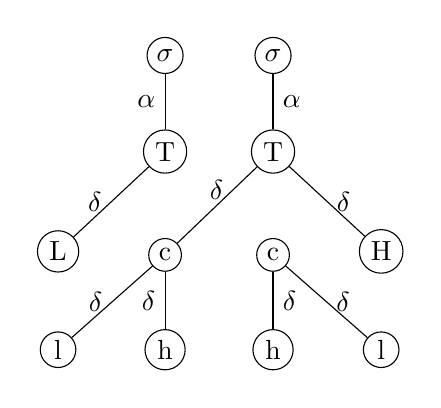
\begin{tikzpicture} [baseline = (y1.base)]
\matrix (m) [matrix of nodes, column sep = 2.3em, row sep = 2em]{
& \node[draw,circle, inner sep =2pt](x1){$\sigma$};  &  \node[draw,circle, inner sep =2pt](x2){$\sigma$};  \\
& \node[draw,circle, inner sep =2pt](y1){T}; &   \node[draw,circle, inner sep =2pt](y2){T}; \\
\node[draw,circle, inner sep =2pt](z1){L}; & \node[draw,circle, inner sep =2pt](z2){c}; &   \node[draw,circle, inner sep =2pt](z3){c}; & \node[draw,circle, inner sep =2pt](z4){H}; \\
\node[draw,circle, inner sep =2pt](t1){l}; & \node[draw,circle, inner sep =2pt](t2){h}; &  \node[draw,circle, inner sep =2pt](t3){h}; & \node[draw,circle, inner sep =2pt](t4){l}; \\
};
\draw (x1) -- (y1) node[left, pos=.5]{$\alpha$};
\draw (x2) -- (y2) node[right, pos=.5]{$\alpha$};
\draw (z1) -- (y1) node[left, pos=.5]{$\delta$};
\draw (z2) -- (y2) node[left, pos=.7]{$\delta$};
\draw (z2) -- (t1) node[left, pos=.5]{$\delta$};
\draw (z2) -- (t2) node[left, pos=.5]{$\delta$};
\draw (y2) -- (z4) node[right, pos=.5]{$\delta$};
\draw (z3) -- (t3) node[right, pos=.5]{$\delta$};
\draw (z3) -- (t4) node[right, pos=.5]{$\delta$};
\end{tikzpicture}
\hspace{1.5cm}
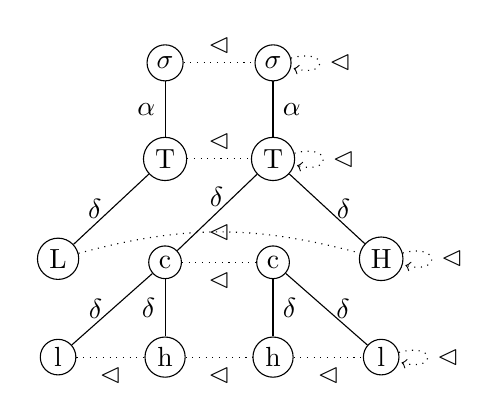
\begin{tikzpicture} [baseline = (y1.base)]
\matrix (m) [matrix of nodes, column sep = 2.3em, row sep = 2em]{
& \node[draw,circle, inner sep =2pt](x1){$\sigma$};  &  \node[draw,circle, inner sep =2pt](x2){$\sigma$};  \\
& \node[draw,circle, inner sep =2pt](y1){T}; &   \node[draw,circle, inner sep =2pt](y2){T}; \\
\node[draw,circle, inner sep =2pt](z1){L}; & \node[draw,circle, inner sep =2pt](z2){c}; &   \node[draw,circle, inner sep =2pt](z3){c}; & \node[draw,circle, inner sep =2pt](z4){H}; \\
\node[draw,circle, inner sep =2pt](t1){l}; & \node[draw,circle, inner sep =2pt](t2){h}; &  \node[draw,circle, inner sep =2pt](t3){h}; & \node[draw,circle, inner sep =2pt](t4){l}; \\
};
\draw (x1) -- (y1) node[left, pos=.5]{$\alpha$};
\draw (x2) -- (y2) node[right, pos=.5]{$\alpha$};
\draw (z1) -- (y1) node[left, pos=.5]{$\delta$};
\draw (z2) -- (y2) node[left, pos=.7]{$\delta$};
\draw (z2) -- (t1) node[left, pos=.5]{$\delta$};
\draw (z2) -- (t2) node[left, pos=.5]{$\delta$};
\draw (y2) -- (z4) node[right, pos=.5]{$\delta$};
\draw (z3) -- (t3) node[right, pos=.5]{$\delta$};
\draw (z3) -- (t4) node[right, pos=.5]{$\delta$};
\draw [dotted] (x1) -- (x2) node[above, pos=.5]{$\vartriangleleft$};
\draw [dotted] (y1) -- (y2) node[above, pos=.5]{$\vartriangleleft$};
\draw [dotted] (t1) -- (t2) node[below, pos=.5]{$\vartriangleleft$};
\draw [dotted] (t2) -- (t3) node[below, pos=.5]{$\vartriangleleft$};
\draw [dotted] (t3) -- (t4) node[below, pos=.5]{$\vartriangleleft$};
\draw [dotted] (z2) -- (z3) node[below, pos=.5]{$\vartriangleleft$};
\path [dotted] (z1) edge [bend left = 15, align = center] node{$\vartriangleleft$} (z4);
\path [dotted] (x2) edge [loop right, align = center] node{$\vartriangleleft$} (x2);
\path [dotted] (y2) edge [loop right, align = center] node{$\vartriangleleft$} (y2);
\path [dotted] (z4) edge [loop right, align = center] node{$\vartriangleleft$} (z4);
\path [dotted] (t4) edge [loop right, align = center] node{$\vartriangleleft$} (t4);
\end{tikzpicture}
\end{center}
Admittedly, this transduction is a bit janky. At least two things stand out about the output. One is that the first syllable seems to be a deformed structure, specifically, it lacks a `c' node. Since Chen analyzes the first syllable as taking a default `l' tone under the c node, one way around this issue is to stipulate the default rule as a result of having no explicitly specified contour (such that it applies in a different module). Another concern is the undominated `c' node from the second syllable. It is fully-specified in terms of the successor function and dominance internally, so why isn't it pronounced? Should it still be there? A possible analysis of this piece of structure is to say that it isn't pronounced because it is not dominated by a T node. In other words, tonal information is only given a phonetic interpretation if a dominance relation exists with a tonal root (T) node. This, of course, needs to be validated. \par
An alternative to this analysis which addresses the second issue (but not the first) is to try to `delete' that piece of structure from the representation. This is done in two steps. The first is to redefine the unary relations such that only the contour of the first syllable appears in the output. This entails new definitions for the `c' node and terminal tonal node relations:\footnote{I'm not sure whether the definitions for $\delta(cf,c)$ and $\delta(T,c)$ work, or whether they need to include the $\land \neg last(x)$ conjuncts. It seems that this is already stipulated in the updated unary function definitions, but since all output relations/functions are defined with respect to the input signature, including these may be necessary.}
\begin{equation}
\begin{aligned}
P^{\tau}_{c}(x)&\myeq P_{c}(x)\,\land\,\neg last(x) \\
P^{\tau}_{l}(x)&\myeq P_{l}(x)\,\land\,\neg last(x) \\
P^{\tau}_{h}(x)&\myeq P_{h}(x)\,\land\,\neg last(succ(x)) \\
\end{aligned}
\end{equation}
 This requires redefining the third disjunct of the dominance function; here, the definition in (\ref{domdef2}) is more appropriate. The revised definition is presented below:
\begin{equation}
\begin{aligned}
\delta^{\tau}(x)=y&\myeq\Big[P_{rf}(x)\land P_{T}(y)\land[\delta(succ(x)) = succ(y)]\Big]\lor \\
&\quad\,\,\Big[P_{cf}(x)\land P_{c}(y)\land[\big(\delta(succ(x))=succ(y)\big)\lor\big(\delta(succ(succ(x)))=succ(y)\big)]\Big]\lor \\
&\quad\,\,\Big[P_{c}(x)\land P_{T}(y)\land last(y)\Big]
\end{aligned}
\end{equation}
The effect of these definitions is to erase the second syllables contour information, resulting in a structure for which the only contour information is that from the first syllable, but which is dominated by the second syllable's `T' node.
\begin{center}
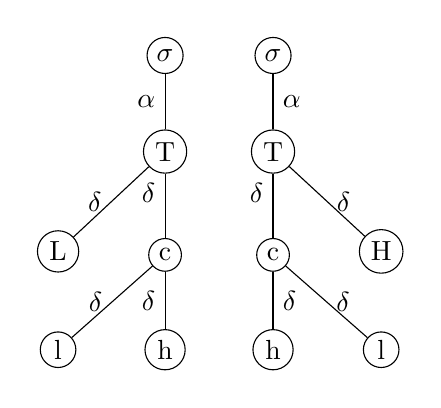
\begin{tikzpicture} [baseline = (y1.base)]
\matrix (m) [matrix of nodes, column sep = 2.3em, row sep = 2em]{
& \node[draw,circle, inner sep =2pt](x1){$\sigma$};  &  \node[draw,circle, inner sep =2pt](x2){$\sigma$};  \\
& \node[draw,circle, inner sep =2pt](y1){T}; &   \node[draw,circle, inner sep =2pt](y2){T}; \\
\node[draw,circle, inner sep =2pt](z1){L}; & \node[draw,circle, inner sep =2pt](z2){c}; &   \node[draw,circle, inner sep =2pt](z3){c}; & \node[draw,circle, inner sep =2pt](z4){H}; \\
\node[draw,circle, inner sep =2pt](t1){l}; & \node[draw,circle, inner sep =2pt](t2){h}; &  \node[draw,circle, inner sep =2pt](t3){h}; & \node[draw,circle, inner sep =2pt](t4){l}; \\
};
\draw (x1) -- (y1) node[left, pos=.5]{$\alpha$};
\draw (x2) -- (y2) node[right, pos=.5]{$\alpha$};
\draw (z1) -- (y1) node[left, pos=.5]{$\delta$};
\draw (z2) -- (y1) node[left, pos=.7]{$\delta$};
\draw (z3) -- (y2) node[left, pos=.7]{$\delta$};
\draw (z2) -- (t1) node[left, pos=.5]{$\delta$};
\draw (z2) -- (t2) node[left, pos=.5]{$\delta$};
\draw (y2) -- (z4) node[right, pos=.5]{$\delta$};
\draw (z3) -- (t3) node[right, pos=.5]{$\delta$};
\draw (z3) -- (t4) node[right, pos=.5]{$\delta$};
\end{tikzpicture}
\hspace{.5cm}
$\rightarrow$
\hspace{.5cm}
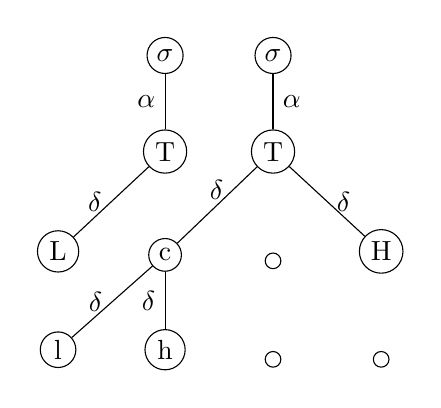
\begin{tikzpicture} [baseline = (y1.base)]
\matrix (m) [matrix of nodes, column sep = 2.3em, row sep = 2em]{
& \node[draw,circle, inner sep =2pt](x1){$\sigma$};  &  \node[draw,circle, inner sep =2pt](x2){$\sigma$};  \\
& \node[draw,circle, inner sep =2pt](y1){T}; &   \node[draw,circle, inner sep =2pt](y2){T}; \\
\node[draw,circle, inner sep =2pt](z1){L}; & \node[draw,circle, inner sep =2pt](z2){c}; &   \node[draw,circle, inner sep =2pt](z3){\hspace{1em}}; & \node[draw,circle, inner sep =2pt](z4){H}; \\
\node[draw,circle, inner sep =2pt](t1){l}; & \node[draw,circle, inner sep =2pt](t2){h}; &  \node[draw,circle, inner sep =2pt](t3){\hspace{1em}}; & \node[draw,circle, inner sep =2pt](t4){\hspace{1em}}; \\
};
\draw (x1) -- (y1) node[left, pos=.5]{$\alpha$};
\draw (x2) -- (y2) node[right, pos=.5]{$\alpha$};
\draw (z1) -- (y1) node[left, pos=.5]{$\delta$};
\draw (z2) -- (y2) node[left, pos=.7]{$\delta$};
\draw (z2) -- (t1) node[left, pos=.5]{$\delta$};
\draw (z2) -- (t2) node[left, pos=.5]{$\delta$};
\draw (y2) -- (z4) node[right, pos=.5]{$\delta$};
\end{tikzpicture}
\end{center} \par
A final question which remains is how to define the successor function, now that three nodes have been deleted. I don't know, but one way to get started on answering this question is to define it in a way similar to the unary predicates.
\begin{equation}
\begin{aligned}
succ^{\tau}(x)\myeq &[P_{c}(x)\land \neg last(x) \land x+1] \lor \\
&[P_{cf}(x) \land \neg last(x) \land \neg pred(last(x)) \land x+1] ????
\end{aligned}
\end{equation}
I will need to address this question of how to define the successor function in both the general model and in transductions.
\end{document}